\begin{frame}{第十四讲、变化率与相对变化率}
	\linespread{1.5}
	\begin{enumerate}
	  \item {\bf 内容与要求}{\b( \S 4.4 )}
	  \begin{itemize}
	    \item 理解变化率与相对变化率的概念
% 	    \begin{itemize}
% 	      \item 了解隐函数和参数方程的高阶导数计算方法
% 	    \end{itemize}
	    \item 掌握与导数相关的应用问题的基本解法
	  \vspace{1em}
	  \end{itemize}
	  \item {\bf 课后练习:}
	  \begin{itemize}
	    \item 书面作业:{\b 习题4.4:6,9,12,14,15,17}
% 	    \item 思考题:{\b 习题4.4:16,17,19;习题4.3:2,9,10,12-14}
	  \end{itemize}
	\end{enumerate}
\end{frame}

\begin{frame}{变化率与导数}
	\linespread{1.2}\pause 
	{\bf 变化率:}一个变量随另一个变量变化过程中,相对于后者发生变化的速率\pause 
	\begin{itemize}
	  \item \alert{速度}:位移关于时间的变化率\pause 
	  \item \alert{密度}:质量关于体积的变化率\pause 
	  \item \alert{电流强度}:电量关于时间的变化率\pause 
	  \item \alert{边际收益}:收益关于投入的变化率\pause 
	  \item \alert{斜率}:线性函数的函数值关于自变量的变化率\pause 
	  \item \alert{\ldots\ldots}\pause 
	\end{itemize}
	{\bf 导数:}对于各种变化率的数学抽象
\end{frame}

\begin{frame}
	\linespread{1.2}
	\begin{exampleblock}{{\bf 例1}\hfill P205-例1}
		考虑运动员进行10m高台跳水的场景。设$t$秒时,运动员相对水面的高度为
		$$H(t)=-4.9t^2+\df{19.6}{3}t+10\;(\mbox{米})$$
		求:
		\begin{enumerate}
		  \item 2秒时运动员的下降速度;
		  \item 运动员起跳后何时上升速度为0;
		  \item 运动员的入水的垂直速度。
		\end{enumerate}
	\end{exampleblock}\pause 
\end{frame}

\begin{frame}
	\linespread{1.5}
	\begin{exampleblock}{{\bf 例2}\hfill P209-例7}
		有一深度$8$m,上底直径$8$m的圆锥形容器,以$4$m$^3$/min的速率向其中注水,
		当容器中水深$5$m时,水面上升的速度是多少?
	\end{exampleblock}
\end{frame}

\begin{frame}
	\linespread{1.5}
	\begin{exampleblock}{{\bf 例3}\hfill P209-例8}
		甲乙两船分别向南和向东航行。在初始时刻,甲船恰位于乙船北方$40$km处,后来在某一时刻测得
		甲船向南航行了20km,此时速度为15km/h;乙船向东航行了15km,此时速度为25km/h。问该时刻
		两船是在相互靠近还是远离,二者的相对速度是多少?
	\end{exampleblock}
\end{frame}

%==========================

\begin{frame}[<+->]{小结}
	\linespread{1.6}
	\begin{block}{{\bf 解题一般步骤}\hfill P210}
		\begin{enumerate}
  		  \item {\ba{ 画图$^*$:}}画出示意图
		  \item {\ba{ 确定变量:}}给出各变量的数学符号表示
		  \item {\ba{ 建立关系:}}根据已知,建立变量关系式
		  \item {\ba{ 求导:}}对所建立的关系式两边求导
		  \item {\ba{ 求解:}}整理新的关系式,得出结果
		\end{enumerate}
	\end{block}
\end{frame}

% \begin{frame}
% 	\linespread{1.2}
% 	\begin{exampleblock}{{\bf 例2}\hfill P211-习题7}
% 	下图包含了沿坐标轴轴线运动物体的位置$s(t)$,速度$v(t)$和加速度$a(t)$的函数图形,试
% 	根据图形特征指出每条曲线对应的函数分别是什么。
% 	\begin{center}
% 		\resizebox{!}{5cm}{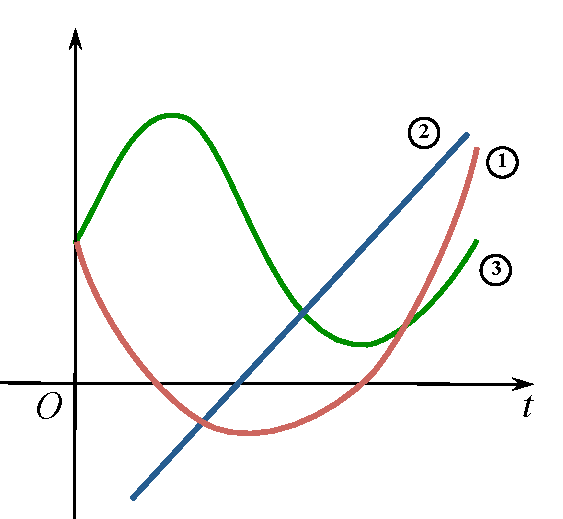
\includegraphics{./images/ch4/ffa.pdf}}
% 	\end{center}
% 	\end{exampleblock}
% \end{frame}

% \begin{frame}{title}
% 	\linespread{1.2}
% 	\begin{block}{{\bf title}\hfill}
% 		123
% 	\end{block}
% \end{frame}